\chapter{Programming}
\section{Hardware Description Languages}
\subsection{Abstraction Levels}
The purpose of using different abstraction levels is to hide details which are not essential for the current view of the problem. Information that is not important is hidden in higher levels of abstraction. The different abstraction levels of HDLs are shown in figure \ref{fig:hdlabstractionlevels}.
\begin{figure}[htbp]
\begin{center}
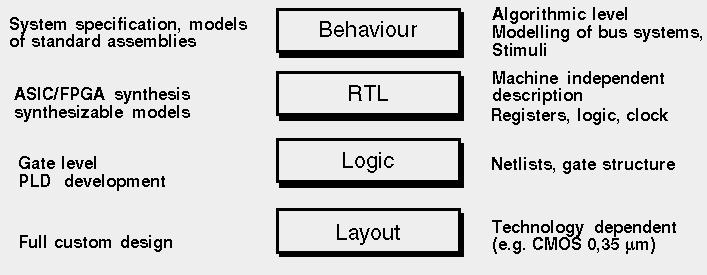
\includegraphics[width=10cm,keepaspectratio=true]{bilder/png/hdlabstractionlevels}
\caption{Abstraction levels of a HDL \cite{Ver16}}
\label{fig:hdlabstractionlevels}
\end{center}
\end{figure}
\subsubsection{Behavioural Level}
The behavioural level describes the behaviour of a system, regarding to its input-output relationships.\cite{Hartenstein1987}. The system is shown defining concurrent algorithms, where each of them is in a sequential manner. The behavioural level is often used to model complete systems. Also stimuli for the RTL-level are described in that level. A point to mention is the fact, that no system clock is defined and signal transitions are asynchronous with respect to the switching time.\\
It must be pointed out, that hardware descriptions in the behavioural level are simulateable, but usually not synthesizable. This means that no hardware manufacturing process can be done using only that description.\cite{Ver16}

\subsubsection{Register-Transfer Level}
\subsubsection{Logical Level}
\subsubsection{Layout Level}
\label{kap:HDL}
\subsection{VHDL}
\subsection{Verilog}